\section{（余）\trCartesianFibration{}}
\label{sec:cocartesian-fibrations}

在本节中，我们定义并讨论\trCartesianFibration{}与\trCocartesianFibration{}的
概念，特别是当 $p\colon X \to Y$ 为\trSimplicialSets{}之间的一个%
\trInnerFibration{}时，$X$ 的 $p$-(余)笛卡尔\trMorphism{}的概念。%
（余）\trCartesianFibration{}分别是\trRightFibration{}与\trLeftFibration{}的%
自然推广，它们将在\trStraightening{}--\trUnstraightening{}%
等价（本书仅在某种程度上讨论该等价）中扮演关键角色。我们将引入（固定基
∞-\trCategory{}上的）\trCartesianFibration{}与\trCocartesianFibration{}之间的%
\trMorphism{}的概念，并证明这类\trMorphism{}中的\trEquivalence{}可以逐纤维地
检测，也就是说，这样的一个\trMorphism{}只要在每个\trFibre{}上诱导的\trFunctor{}%
是\trEquivalence{}，它本身就已经是\trEquivalence{}。在经典的\trCategoryTheory{}%
中，\trCartesianFibration{}与\trCocartesianFibration{}以格罗滕迪克-(op)-纤维化
（Grothendieck-(op)-fibration）之名为人所知；在格罗滕迪克构造下，它们作为取值于%
\trCategories{}的 2-范畴中的（伪）\trFunctor{}的伴随物而出现。

\begin{definition}\label{def:p-cartesian-morphism}
设 $p\colon X \to Y$ 是\trSimplicialSets{}之间的一个\trInnerFibration{}。\trMorphism{}%
$f\colon \Delta^1 \to X$ 称为 \emph{$p$-笛卡尔的}（$p$-cartesian），如果对
$n \ge 2$，任何形如下述图表的\trLiftingProblem{}%
\begin{center}
\begin{tikzpicture}
  \node (dn1) at (0,0) {$\Delta^{(n-1,n)}$};
  \node (horn) at (3,0) {$\Lambda^n_n$};
  \node (x) at (5.8,0) {$X$};
  \node (dn) at (3,-1.8) {$\Delta^n$};
  \node (y) at (5.8,-1.8) {$Y$};
  \draw[->] (dn1) -- (horn);
  \draw[->] (horn) -- (x);
  \draw[->] (horn) -- (dn);
  \draw[->] (x) -- (y);
  \draw[->] (dn) -- (y);
  \draw[->, dashed] (dn) -- (x);
  \draw[->, bend left=25] (dn1) to node[above] {$f$} (x);
\end{tikzpicture}
\end{center}
容有一个解。对偶地，称它为 \emph{$p$-余笛卡尔的}（$p$-cocartesian），如果任何
形如下述图表的\trLiftingProblem{}%
\begin{center}
\begin{tikzpicture}
  \node (d01) at (0,0) {$\Delta^{(0,1)}$};
  \node (horn) at (3,0) {$\Lambda^n_0$};
  \node (x) at (5.8,0) {$X$};
  \node (dn) at (3,-1.8) {$\Delta^n$};
  \node (y) at (5.8,-1.8) {$Y$};
  \draw[->] (d01) -- (horn);
  \draw[->] (horn) -- (x);
  \draw[->] (horn) -- (dn);
  \draw[->] (x) -- (y);
  \draw[->] (dn) -- (y);
  \draw[->, dashed] (dn) -- (x);
  \draw[->, bend left=25] (d01) to node[above] {$f$} (x);
\end{tikzpicture}
\end{center}
容有一个解。人们称这样的一个 $f$ 为 $p(f)$ 的一个 $p$-(余)笛卡尔提升。
\end{definition}

（余）笛卡尔\trMorphism{}的定义可以借\trSlice{}的语言重新表述如下。

\begin{lemma}\label{lem:cartesian-slice-criterion}
设 $p\colon X \to Y$ 是一个\trInnerFibration{}，并设 $f\colon x \to y$ 是 $X$
中的一个\trMorphism{}。\footnote{译注：原书印作「$Y$ 中的一个态射」，按上下文
应为 $X$，此处径改。——译者注}那么，$f$ 是 $p$-笛卡尔的，当且仅当\trFunctor{}%
\[
X_{/f} \longrightarrow X_{/y} \times_{Y_{/p(y)}} Y_{/pf}
\]
是一个\trTrivialFibration{}。对偶地，$f$ 是 $p$-余笛卡尔的，当且仅当\trFunctor{}%
\[
X_{f/} \longrightarrow X_{x/} \times_{Y_{p(x)/}} Y_{pf/}
\]
是一个\trTrivialFibration{}。
\end{lemma}

\begin{proof}
设 $n \ge 0$，考虑\trLiftingProblem{}%
\begin{center}
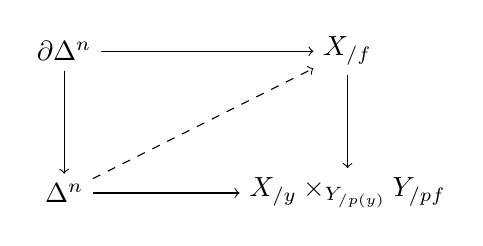
\begin{tikzpicture}
  \node (bd) at (0,0) {$\partial\Delta^n$};
  \node (xf) at (3.6,0) {$X_{/f}$};
  \node (dn) at (0,-1.8) {$\Delta^n$};
  \node (pb) at (3.6,-1.8) {$X_{/y} \times_{Y_{/p(y)}} Y_{/pf}$};
  \draw[->] (bd) -- (xf);
  \draw[->] (bd) -- (dn);
  \draw[->] (xf) -- (pb);
  \draw[->] (dn) -- (pb);
  \draw[->, dashed] (dn) -- (xf);
\end{tikzpicture}
\end{center}
我们希望求解它。经\trAdjunction{}，它对应于\trLiftingProblem{}%
\begin{center}
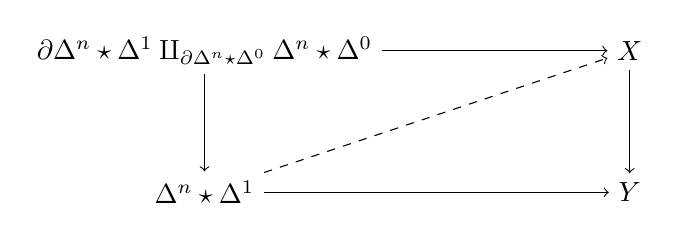
\begin{tikzpicture}
  \node (po) at (0,0)
    {$\partial\Delta^n \star \Delta^1 \amalg_{\partial\Delta^n \star \Delta^0} \Delta^n \star \Delta^0$};
  \node (x) at (5.4,0) {$X$};
  \node (dj) at (0,-1.8) {$\Delta^n \star \Delta^1$};
  \node (y) at (5.4,-1.8) {$Y$};
  \draw[->] (po) -- (x);
  \draw[->] (po) -- (dj);
  \draw[->] (x) -- (y);
  \draw[->] (dj) -- (y);
  \draw[->, dashed] (dj) -- (x);
\end{tikzpicture}
\end{center}
其中在 $\Delta^1$ 上的限制由 $f$ 给出。我们回忆，左边的竖直映射同构于
$\Lambda^{n+2}_{n+2} \to \Delta^{n+2}$，而 $\Delta^1$ 向 $\Lambda^{n+2}_{n+2}$
中的包含就是边 $\Delta^{(n+1,n+2)}$。因此，该图表对一切 $n \ge 0$ 都可解。
余笛卡尔的情形类似。
\end{proof}

\begin{remark}\label{rem:cartesian-slices}
设 $p\colon X \to Y$ 是∞-\trCategories{}之间的一个\trInnerFibration{}。那么，由
第 2 章中的\cref{prop:slice-fat-slice-joyal-equivalence}，对任何图表
$p\colon W \to X$，映射 $X_{/p} \to X^{/p}$ 是一个\trJoyalEquivalence{}%
\footnote{译注：原书在此将 $p$ 两用——既指本注开头的\trInnerFibration{}%
$p\colon X \to Y$，又指任意的图表 $p\colon W \to X$；记号 $X_{/p}$ 与
$X^{/p}$ 中的 $p$ 指后者。——译者注}。此外，映射
\[
X^{/f} \longrightarrow X^{/y} \times_{Y_{/p(y)}} Y^{/pf}
\]
由第 2 章中的\cref{lem:fat-slice-fibration} 也是一个\trRightFibration{}。
（我们仅对 $p$ 为\trIsofibration{}的情形证明过这一点，但见
\cref{rem:fat-slice-inner-fibration}。）因此，$f$ 是笛卡尔的，当且仅当该映射
是一个\trTrivialFibration{}。同样地，$f$ 是余笛卡尔的，当且仅当映射
\[
X^{f/} \longrightarrow X^{x/} \times_{Y^{p(x)/}} Y^{pf/}
\]
是一个\trTrivialFibration{}。
\end{remark}

\begin{lemma}\label{lem:cartesian-composition}
设 $p\colon \E \to \D$ 与 $q\colon \D \to \C$ 是∞-\trCategories{}之间的%
\trInnerFibration{}，并设 $f\colon \Delta^1 \to \E$ 是 $\E$ 中的一个%
\trMorphism{}，使得 $p(f)$ 是 $q$-(余)笛卡尔的。那么，$f$ 是
$p$-(余)笛卡尔的，当且仅当 $f$ 是 $qp$-(余)笛卡尔的。
\end{lemma}

\begin{proof}
考虑图表
\begin{center}
\begin{tikzpicture}
  \node (ef) at (0,0) {$\E_{/f}$};
  \node (mid) at (3.9,0) {$\E_{/y} \times_{\D_{/p(y)}} \D_{/pf}$};
  \node (top) at (11.2,0)
    {$\E_{/y} \times_{\D_{/p(y)}} \D_{/p(y)} \times_{\C_{/q(p(y))}} \C_{/qpf}$};
  \node (bot) at (11.2,-2) {$\E_{/y} \times_{\C_{/q(p(y))}} \C_{/qpf}$};
  \draw[->] (ef) -- (mid);
  \draw[->] (mid) -- node[above] {$\cong$} (top);
  \draw[->] (top) -- node[right] {$\cong$} (bot);
  \draw[->] (ef) -- (bot);
\end{tikzpicture}
\end{center}
其中第二个水平映射由 $pf$ 是 $q$-笛卡尔的这一假设而知是\trTrivialFibration{}。
第一个水平映射与对角映射都是\trRightFibration{}，从而当且仅当它们是%
\trJoyalEquivalence{}时才是\trTrivialFibration{}。引理由此得证。
\end{proof}

\begin{remark}\label{rem:cartesian-composition-general}
前一个引理在去掉所涉\trSimplicialSets{}皆为∞-\trCategories{}的假设后仍然更
一般地成立，见 \cite[Proposition 2.4.1.3]{Lur09}：由于\trTrivialFibration{}的复合
仍是\trTrivialFibration{}，我们立即看到，若 $f$ 是 $p$-笛卡尔的，则它也是
$qp$-笛卡尔的。为了看出其逆，我们可以证明映射
$\E_{/f} \to \E_{/y} \times_{\D_{/p(y)}} \D_{/pf}$（由\trThreeForTwoProperty{}，
它是\trJoyalEquivalence{}）实际上具有可缩的\trFibre{}，然后诉诸下述一般事实：
具有可缩\trFibre{}的\trRightFibration{}是一个\trTrivialFibration{}（或者说是%
\trJoyalEquivalence{}，从而是\trTrivialFibration{}），见 \cite[Lemma 2.1.3.4]{Lur09} 或\cref{thm:fibrewise-criterion}。我们所关心的%
\trFibre{}是另外两个映射各自的\trFibre{}之间的那个映射的\trFibre{}。由于这些%
\trFibre{}按假设是可缩的，即得断言。
\end{remark}

\begin{lemma}\label{lem:equivalence-cartesian}
设 $p\colon \E \to \C$ 是∞-\trCategories{}之间的一个\trInnerFibration{}，并设
$f\colon \Delta^1 \to \E$ 是一个\trMorphism{}。那么，$f$ 是一个\trEquivalence{}，
当且仅当 $f$ 是 $p$-(余)笛卡尔的且 $p(f)$ 是一个\trEquivalence{}。
\end{lemma}

\begin{proof}
设 $f$ 是一个\trEquivalence{}。那么 $p(f)$ 亦然，而\trJoyal{}提升定理（第 2 章
中的\cref{thm:special-horn-lifting}）蕴含 $f$ 既是笛卡尔的又是余笛卡尔的。反之，
现在设 $p(f)$ 是一个\trEquivalence{}，从而由\cref{ex:p-cocartesian-over-point}（取 $q\colon \C \to \Delta^0$
为投影）它是 $q$-笛卡尔的。由\cref{lem:cartesian-composition}，我们发现 $f$ 是
$p$-笛卡尔的，当且仅当 $f$ 是 $qp$-笛卡尔的；而由\cref{ex:p-cocartesian-over-point}的再一次应用，后者
当且仅当 $f$ 是一个\trEquivalence{}时成立。
\end{proof}

\begin{lemma}\label{lem:cartesian-three-for-two}
设 $p\colon \E \to \C$ 是一个\trInnerFibration{}，并设 $\sigma\colon \Delta^2 \to \E$，
我们把它描绘成图表
\begin{center}
\begin{tikzpicture}
  \node (y) at (2.2,0) {$y$};
  \node (x) at (0,-1.8) {$x$};
  \node (z) at (4.4,-1.8) {$z$};
  \draw[->] (x) -- node[above, pos=0.35] {$f$} (y);
  \draw[->] (y) -- node[above right, pos=0.4] {$\varphi$} (z);
  \draw[->] (x) -- node[below] {$g$} (z);
\end{tikzpicture}
\end{center}
设 $\varphi$ 是 $p$-笛卡尔的。那么，$g$ 是 $p$-笛卡尔的，当且仅当 $f$ 是
$p$-笛卡尔的。
\end{lemma}

\begin{proof}
我们观察到，包含 $\Delta^{(0,1)} \to \Delta^2$ 与 $\Delta^{(0,2)} \to \Delta^2$
都是左零调的，于是在两个交换方块
\begin{center}
\begin{tikzpicture}
  \node (tl) at (0,0) {$\E_{/\sigma}$};
  \node (tr) at (4.2,0) {$\E_{/z} \times_{\C_{/p(z)}} \C_{/p\sigma}$};
  \node (bl) at (0,-1.8) {$\E_{/g}$};
  \node (br) at (4.2,-1.8) {$\E_{/z} \times_{\C_{/p(z)}} \C_{/pg}$};
  \draw[->] (tl) -- (tr);
  \draw[->] (tl) -- (bl);
  \draw[->] (tr) -- (br);
  \draw[->] (bl) -- (br);
\end{tikzpicture}
\qquad
\begin{tikzpicture}
  \node (tl) at (0,0) {$\E_{/\sigma}$};
  \node (tr) at (4.2,0) {$\E_{/y} \times_{\C_{/p(y)}} \C_{/p\sigma}$};
  \node (bl) at (0,-1.8) {$\E_{/f}$};
  \node (br) at (4.2,-1.8) {$\E_{/y} \times_{\C_{/p(y)}} \C_{/pf}$};
  \draw[->] (tl) -- (tr);
  \draw[->] (tl) -- (bl);
  \draw[->] (tr) -- (br);
  \draw[->] (bl) -- (br);
\end{tikzpicture}
\end{center}
中，所有竖直映射都是\trTrivialFibration{}。我们希望证明：左下方的水平映射是
一个\trTrivialFibration{}，当且仅当右下方的水平映射是。由于这两个映射无论如
何都是\trIsofibration{}，故只需证明：一个映射是\trJoyalEquivalence{}当且仅当
另一个映射是。借助这两个交换方块，从而只需证明：左上方的水平映射是%
\trJoyalEquivalence{}当且仅当右上方的水平映射是。为此，我们考虑图表
\begin{center}
\begin{tikzpicture}
  \node (top) at (5.4,0.9) {$\E_{/\sigma}$};
  \node (left) at (0,-1.1) {$\E_{/y} \times_{\C_{/p(y)}} \C_{/p\sigma}$};
  \node (middle) at (5.4,-1.1) {$\E_{/\varphi} \times_{\C_{/p\varphi}} \C_{/p\sigma}$};
  \node (right) at (11.2,-1.1) {$\E_{/z} \times_{\C_{/p(z)}} \C_{/p\sigma}$};
  \draw[->] (top) to[bend right=20] (left);
  \draw[->] (top) -- (middle);
  \draw[->] (top) to[bend left=20] (right);
  \draw[->] (middle) -- node[above] {$\cong$} (right);
  \draw[<-] (left) -- node[below] {$\cong$} (middle);
\end{tikzpicture}
\end{center}
这里，右边的水平映射是一个\trEquivalence{}，因为 $\varphi$ 是 $p$-笛卡尔的，
从而映射 $\E_{/\varphi} \to \E_{/z} \times_{\C_{/p(z)}} \C_{/p\varphi}$ 是一个%
\trEquivalence{}。左边的水平映射是一个\trEquivalence{}，因为它由限制
$\{1\} \to \Delta^{(1,2)}$ 诱导，而后者是左零调的。因此，我们发现左边的弯映射
是一个\trEquivalence{}当且仅当右边的弯映射是一个\trEquivalence{}，此即尚待
证明者。
\end{proof}

\begin{remark}\label{rem:cartesian-three-for-two-base}
\cref{lem:cartesian-three-for-two} 的结论并不要求基 $\C$ 是一个∞-\trCategory{}。
事实上，一旦建立了更一般的概念——\trLocallyCocartesian{}边（locally
cocartesian edge）——的若干性质，这一化归并不算太复杂，见 \cite[2.4.2]{Lur09} 与定义 3.2.5 之后的讨论。
\end{remark}

下述概念用起来会带来便利。

\begin{definition}\label{def:cartesian-fibration}
∞-\trCategories{}的一个交换图表
\begin{center}
\begin{tikzpicture}
  \node (tl) at (0,0) {$\E$};
  \node (tr) at (2.6,0) {$\E'$};
  \node (bl) at (0,-1.8) {$\C$};
  \node (br) at (2.6,-1.8) {$\C'$};
  \draw[->] (tl) -- (tr);
  \draw[->] (tl) -- (bl);
  \draw[->] (tr) -- node[right] {$p$} (br);
  \draw[->] (bl) -- (br);
\end{tikzpicture}
\end{center}
称为\emph{同伦笛卡尔的}（homotopy-cartesian），如果 $p$ 是一个\trIsofibration{}，
且诱导映射 $\E \to \C \times_{\C'} \E'$ 是一个\trJoyalEquivalence{}。对
$\C = \Delta^0$，我们对复合 $\E \to \E' \to \C'$ 也将使用%
\emph{\trHomotopy{}\trFibreSequence{}}（homotopy fibre sequence）一词。
\end{definition}

\begin{remark}\label{rem:homotopy-cartesian-drop-isofibration}
更一般地，可以通过把 $p$ 分解为一个\trJoyalEquivalence{}后接一个%
\trIsofibration{}%
\[
\E' \xrightarrow{\ \simeq\ } \E'' \xrightarrow{\ q\ } \C'
\]
来省去 $p$ 为\trIsofibration{}这一条件，然后要求诱导映射
$\E \to \C \times_{\C'} \E''$ 是一个\trJoyalEquivalence{}。
\end{remark}

\begin{lemma}\label{lem:isofibration-mapping-space-kan}
设 $p\colon \C \to \D$ 是∞-\trCategories{}之间的一个\trIsofibration{}，并设 $x$
与 $y$ 是 $\C$ 的\trObject{}。那么诱导映射
\[
\mathrm{map}_{\C}(x, y) \longrightarrow \mathrm{map}_{\D}(p(x), p(y))
\]
是一个\trKanFibration{}。对于 $\mathrm{map}^L$ 与 $\mathrm{map}^R$，同样的断言
成立，即使 $p$ 只是一个\trInnerFibration{}。
\end{lemma}

\begin{proof}
我们考虑图表
\begin{center}
\begin{tikzpicture}
  \node (ml) at (0,0) {$\mathrm{map}_{\C}(x, y)$};
  \node (mm) at (4.6,0) {$\mathrm{map}_{\D}(p(x), p(y))$};
  \node (mr) at (9.2,0) {$\Delta^0$};
  \node (cl) at (0,-1.7) {$\C^{/y}$};
  \node (cm) at (4.6,-1.7) {$\D_{/p(y)} \times_{\D} \C$};
  \node (cr) at (9.2,-1.7) {$\C$};
  \node (bm) at (4.6,-3.4) {$\D_{/p(y)}$};
  \node (br) at (9.2,-3.4) {$\D$};
  \draw[->] (ml) -- (mm);
  \draw[->] (mm) -- (mr);
  \draw[->] (ml) -- (cl);
  \draw[->] (mm) -- (cm);
  \draw[->] (mr) -- node[right] {$x$} (cr);
  \draw[->] (cl) -- (cm);
  \draw[->] (cm) -- (cr);
  \draw[->] (cm) -- (bm);
  \draw[->] (cr) -- node[right] {$p$} (br);
  \draw[->] (bm) -- (br);
\end{tikzpicture}
\end{center}
或分别考虑用通常切片 $\C_{/y}$ 替代 $\C^{/y}$ 的那些图表，以及用 $\C_{x/}$
替代 $\C^{/y}$ 的变体。在该图表中，所有方块都是\trPullback{}：下面那个按定义
是\trPullback{}，右边的大方块同样按定义是，从而右上角的小方块亦然；合并起来的
水平大方块按定义是，从而左边的小方块亦然。下面的水平映射是一个%
\trRightFibration{}（在 $\C_{x/}$ 的情形，它是一个\trLeftFibration{}），故上面
的水平映射亦然。由于 $\mathrm{map}_{\D}(p(x), p(y))$ 是一个\trKanComplex{}，
它实际上是一个\trKanFibration{}，正如所断言的。
\end{proof}

\begin{lemma}\label{lem:fibre-pullback-mapping}
设 $\C \to \D$ 是∞-\trCategories{}之间的一个\trIsofibration{}，设 $z$ 是 $\D$
的一个\trObject{}，并设 $x$ 与 $y$ 是 $\C$ 的满足 $p(x) = p(y) = z$ 的\trObject{}。
那么图表
\begin{center}
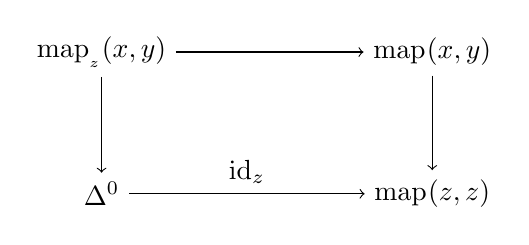
\begin{tikzpicture}
  \node (tl) at (0,0) {$\mathrm{map}_{\C_z}(x, y)$};
  \node (tr) at (4.2,0) {$\mathrm{map}_{\C}(x, y)$};
  \node (bl) at (0,-1.8) {$\Delta^0$};
  \node (br) at (4.2,-1.8) {$\mathrm{map}_{\D}(z, z)$};
  \draw[->] (tl) -- (tr);
  \draw[->] (tl) -- (bl);
  \draw[->] (tr) -- (br);
  \draw[->] (bl) -- node[above] {$\mathrm{id}_z$} (br);
\end{tikzpicture}
\end{center}
是一个\trPullback{}。
\end{lemma}

\begin{proof}
为了看出剩下的断言，我们考虑图表
\begin{center}
\begin{tikzpicture}
  \node (fxy) at (3.4,8.4) {$F_{x,y}$};
  \node (mxy) at (8.8,8.4) {$\mathrm{map}_{\E}(x, y)$};
  \node (mzz) at (14.4,8.4) {$\mathrm{map}_{\C}(z, z)$};
  \node (e1z) at (1.1,5.4) {$\E^{\Delta^1}_z$};
  \node (e1) at (6.4,5.4) {$\E^{\Delta^1}$};
  \node (c1) at (12,5.4) {$\C^{\Delta^1}$};
  \node (d0a) at (3.7,3.2) {$\Delta^0$};
  \node (d0b) at (9,3.2) {$\Delta^0$};
  \node (d0c) at (14.6,3.2) {$\Delta^0$};
  \node (ez) at (1,0) {$\E_z \times \E_z$};
  \node (ee) at (6.3,0) {$\E \times \E$};
  \node (cc) at (11.9,0) {$\C \times \C$};
  \draw[->] (fxy) -- (mxy);
  \draw[->] (mxy) -- (mzz);
  \draw[->] (fxy) -- (d0a);
  \draw[->] (mxy) -- (d0b);
  \draw[->] (mzz) -- (d0c);
  \draw[->] (fxy) -- (e1z);
  \draw[->] (mxy) -- (e1);
  \draw[->] (mzz) -- (c1);
  \draw[->] (e1z) -- (e1);
  \draw[->] (e1) -- (c1);
  \draw[->] (e1z) -- (ez);
  \draw[->] (e1) -- (ee);
  \draw[->] (c1) -- (cc);
  \draw[->] (d0a) -- (d0b);
  \draw[->] (d0b) -- (d0c);
  \draw[->] (d0a) -- (ez);
  \draw[->] (d0b) -- (ee);
  \draw[->] (d0c) -- (cc);
  \draw[->] (ez) -- (ee);
  \draw[->] (ee) -- (cc);
\end{tikzpicture}
\end{center}
其中所有水平复合都由在对应于 $\mathrm{id}_z$ 的那个点上的纤维包含给出。由于
中间的竖直方块与右边的竖直方块都是\trPullback{}，最左边的竖直方块也是%
\trPullback{}。
\end{proof}

\begin{corollary}\label{cor:mapping-homotopy-cartesian}
设 $\C \to \D$ 是∞-\trCategories{}之间的一个\trIsofibration{}，设 $z$ 是 $\D$
的一个\trObject{}，并设 $x$ 与 $y$ 是 $\C_z$ 的\trObject{}。那么图表
\begin{center}
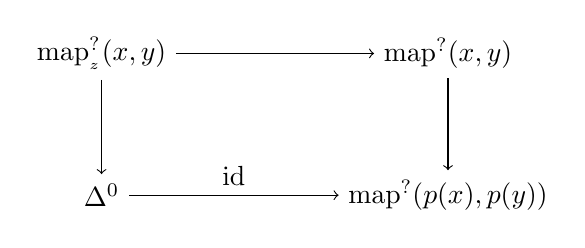
\begin{tikzpicture}
  \node (tl) at (0,0) {$\mathrm{map}^{?}_{\C_z}(x, y)$};
  \node (tr) at (4.4,0) {$\mathrm{map}^{?}_{\C}(x, y)$};
  \node (bl) at (0,-1.8) {$\Delta^0$};
  \node (br) at (4.4,-1.8) {$\mathrm{map}^{?}_{\D}(p(x), p(y))$};
  \draw[->] (tl) -- (tr);
  \draw[->] (tl) -- (bl);
  \draw[->] (tr) -- (br);
  \draw[->] (bl) -- node[above] {$\mathrm{id}$} (br);
\end{tikzpicture}
\end{center}
对 $? = R$、$L$ 或空缺都是同伦笛卡尔的。\footnote{译注：原书此图中右上角印作
$\mathrm{map}^{?}_{\E}(x, y)$、右下角印作 $\mathrm{map}^{?}_{\C}(p(x), p(y))$，
与本推论开头的\trIsofibration{} $\C \to \D$ 不符（$\E$ 未在本推论中出现，且
$p(x),p(y)$ 落在 $\D$ 中）；当系作者沿袭此前 $\E \to \C$ 记号之笔误，兹按上下文
改为 $\mathrm{map}^{?}_{\C}(x, y)$ 与 $\mathrm{map}^{?}_{\D}(p(x), p(y))$。
——译者注}
\end{corollary}

\begin{proof}
对于通常的映射空间，由于该图表是一个\trPullback{}且右边的竖直映射是一个%
\trKanFibration{}，断言立得。为了看出关于右映射空间与左映射空间的断言，我们
使用\cref{lem:isofibration-mapping-space-kan} 与第 2 章中的%
\cref{cor:mapping-space-homotopy-equivalence}。
\end{proof}

\begin{lemma}\label{lem:cartesian-fibre-trivial-fibration}
设 $p\colon \E \to \C$ 是∞-\trCategories{}之间的一个\trInnerFibration{}，并设
$f\colon \Delta^1 \to \E$ 是一个从 $x$ 到 $y$ 的 $p$-笛卡尔\trMorphism{}。那么，
对 $\E$ 的一切\trObject{} $z$，诱导映射
\[
\E^{/f} \times_{\E} \{z\} \longrightarrow
\bigl(\E^{/y} \times_{\C_{/p(y)}} \C^{/pf}\bigr) \times_{\E} \{z\}
\]
也是一个\trTrivialFibration{}。
\end{lemma}

\begin{proof}
我们有交换图表
\begin{center}
\begin{tikzpicture}
  \node (tl) at (0,0) {$\E^{/f} \times_{\E} \{z\}$};
  \node (tr) at (6.4,0) {$\E^{/f}$};
  \node (ml) at (0,-1.8)
    {$\bigl(\E^{/y} \times_{\C_{/p(y)}} \C^{/pf}\bigr) \times_{\E} \{z\}$};
  \node (mr) at (6.4,-1.8) {$\E^{/y} \times_{\C_{/p(y)}} \C^{/pf}$};
  \node (bl) at (0,-3.6) {$\Delta^0$};
  \node (br) at (6.4,-3.6) {$\E$};
  \draw[->] (tl) -- (tr);
  \draw[->] (ml) -- (mr);
  \draw[->] (bl) -- (br);
  \draw[->] (tl) -- (ml);
  \draw[->] (tr) -- (mr);
  \draw[->] (ml) -- (bl);
  \draw[->] (mr) -- (br);
\end{tikzpicture}
\end{center}
其中大方块与下面的方块都是\trPullback{}。于是，上面的方块也是\trPullback{}。
由于在该方块中，右边的竖直映射由 $f$ 是 $p$-笛卡尔的这一假设而知是一个%
\trTrivialFibration{}，断言得证。
\end{proof}

\begin{remark}\label{rem:cartesian-ordinary-slice}
把胖切片换成通常切片，同样的断言对任意\trSimplicialSets{}之间的%
\trInnerFibration{}成立。
\end{remark}

\begin{corollary}\label{cor:cartesian-map-into-fibre}
设 $p\colon \E \to \C$ 是∞-\trCategories{}之间的一个\trInnerFibration{}，设
$f\colon \Delta^1 \to \E$ 是 $\E$ 的一个从 $x$ 到 $y$ 的 $p$-笛卡尔%
\trMorphism{}，并设 $z$ 是 $\E$ 的一个\trObject{}。那么图表
\begin{center}
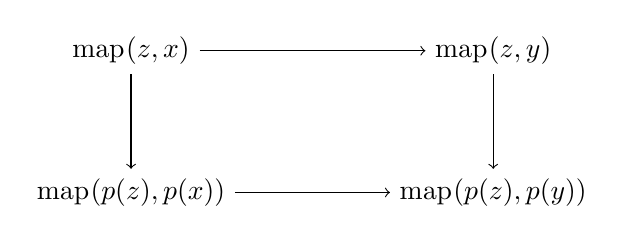
\begin{tikzpicture}
  \node (tl) at (0,0) {$\mathrm{map}_{\E}(z, x)$};
  \node (tr) at (4.6,0) {$\mathrm{map}_{\E}(z, y)$};
  \node (bl) at (0,-1.8) {$\mathrm{map}_{\C}(p(z), p(x))$};
  \node (br) at (4.6,-1.8) {$\mathrm{map}_{\C}(p(z), p(y))$};
  \draw[->] (tl) -- (tr);
  \draw[->] (tl) -- (bl);
  \draw[->] (tr) -- (br);
  \draw[->] (bl) -- (br);
\end{tikzpicture}
\end{center}
是一个由∞-\trGroupoid{}构成的同伦笛卡尔图表。两个水平映射分别由与 $f$ 及
$pf$ 的后复合诱导。
\end{corollary}

\begin{proof}
我们考虑图表
\begin{center}
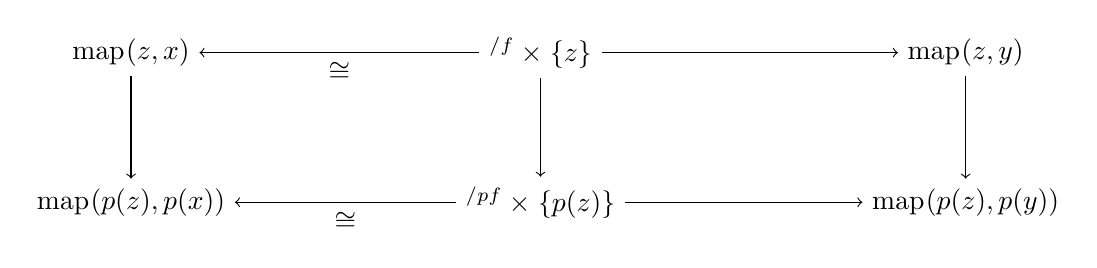
\begin{tikzpicture}
  \node (ml) at (0,0) {$\mathrm{map}_{\E}(z, x)$};
  \node (mm) at (5.2,0) {$\E^{/f} \times_{\E} \{z\}$};
  \node (mr) at (10.6,0) {$\mathrm{map}_{\E}(z, y)$};
  \node (bl) at (0,-1.9) {$\mathrm{map}_{\C}(p(z), p(x))$};
  \node (bm) at (5.2,-1.9) {$\C^{/pf} \times_{\C} \{p(z)\}$};
  \node (br) at (10.6,-1.9) {$\mathrm{map}_{\C}(p(z), p(y))$};
  \draw[<-] (ml) -- node[below] {$\cong$} (mm);
  \draw[->] (mm) -- (mr);
  \draw[->] (ml) -- (bl);
  \draw[->] (mm) -- (bm);
  \draw[->] (mr) -- (br);
  \draw[<-] (bl) -- node[below] {$\cong$} (bm);
  \draw[->] (bm) -- (br);
\end{tikzpicture}
\end{center}
并观察到左边的水平映射都是\trTrivialFibration{}，因为包含 $\{0\} \to \Delta^1$
是左零调的。于是，只需证明右边的方块是同伦笛卡尔的；而由%
\cref{lem:isofibration-mapping-space-kan}，右边的竖直映射是一个%
\trKanFibration{}，故只需回忆映射
\[
\E^{/f} \longrightarrow \E^{/y} \times_{\C_{/p(y)}} \C^{/pf}
\]
是一个\trTrivialFibration{}，从而在施加 $- \times_{\E} \{z\}$ 之后同样的结论
仍然成立。
\end{proof}

\begin{remark}\label{rem:cartesian-map-not-commutative}
\cref{cor:cartesian-map-into-fibre} 的陈述并不完全正确，因为我们构造的那个方块
并不先验地交换（只在同伦意义下交换）。但由于右边的竖直映射是一个%
\trKanFibration{}，它总能在不改变各参与方的同伦型的前提下被换成交换图表，而一个
具体的做法就是考虑上面证明中出现的图表里右边的那个方块。
\end{remark}

\begin{remark}\label{rem:cartesian-characterization}
给定一个\trInnerFibration{} $p\colon \E \to \C$ 和一个\trMorphism{}%
$f\colon \Delta^1 \to \E$，使得对 $\E$ 的\emph{每个}\trObject{} $z$，图表
\begin{center}
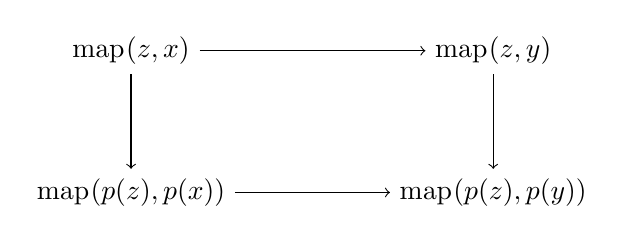
\begin{tikzpicture}
  \node (tl) at (0,0) {$\mathrm{map}_{\E}(z, x)$};
  \node (tr) at (4.6,0) {$\mathrm{map}_{\E}(z, y)$};
  \node (bl) at (0,-1.8) {$\mathrm{map}_{\C}(p(z), p(x))$};
  \node (br) at (4.6,-1.8) {$\mathrm{map}_{\C}(p(z), p(y))$};
  \draw[->] (tl) -- (tr);
  \draw[->] (tl) -- (bl);
  \draw[->] (tr) -- (br);
  \draw[->] (bl) -- (br);
\end{tikzpicture}
\end{center}
是同伦笛卡尔的，则 $f$ 是 $p$-笛卡尔的。这可以通过观察映射
\[
\E^{/f} \longrightarrow \E^{/y} \times_{\C_{/p(y)}} \C^{/pf}
\]
而看出：它是一个\trTrivialFibration{}，当且仅当它在 $\E$ 的各个点之上的每根%
\trFibre{}上都诱导\trEquivalence{}。如前所述，经由一个组合论证，这一断言对%
\trRightFibration{}一般地成立（无需 $\E$ 与 $\C$ 是∞-\trCategories{}）。在
$\E$ 与 $\C$ 为∞-\trCategories{}的情形，我们即将对所谓的\trCartesianFibration{}%
证明这一结果（见\cref{thm:fibrewise-criterion}），随后我们将
从中导出关于\trRightFibration{}的版本。\footnote{译注：原书此式印作
$\E_{/f} \to \E^{/y} \times_{\C^{/(y)}} \C^{/pf}$，有两处笔误：其一，拉回脚标
$\C^{/(y)}$ 脱漏 $p$ 且上下标位置有误；其二，源头 $\E_{/f}$ 是通常切片，与目标
中的胖切片 $\E^{/y}$、$\C^{/pf}$ 混用，与本节平行诸式（\cref{lem:cartesian-slice-criterion}
与\cref{rem:cartesian-slices}）不合。按\cref{rem:cartesian-slices} 所论之映射
（「$f$ 是笛卡尔的，当且仅当该映射是\trTrivialFibration{}」正为本注此处所引者），
兹改为 $\E^{/f} \to \E^{/y} \times_{\C_{/p(y)}} \C^{/pf}$。——译者注}
\end{remark}

\begin{corollary}\label{cor:cartesian-lift-mapping-fibre}
设 $p\colon \E \to \C$ 是一个\trInnerFibration{}，并设 $x$ 与 $y$ 是 $\E$ 的%
\trObject{}。设 $f\colon x' \to y$ 是一个满足 $p(x') = p(x)$ 的 $p$-笛卡尔%
\trMorphism{}。那么图表
\begin{center}
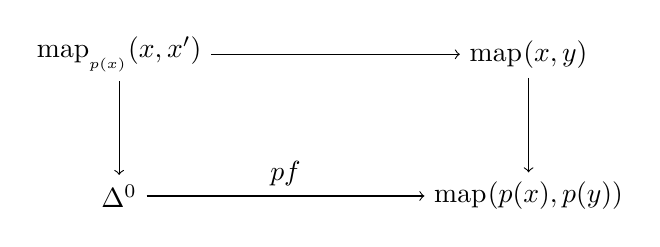
\begin{tikzpicture}
  \node (tl) at (0,0) {$\mathrm{map}_{\E_{p(x)}}(x, x')$};
  \node (tr) at (5.2,0) {$\mathrm{map}_{\E}(x, y)$};
  \node (bl) at (0,-1.8) {$\Delta^0$};
  \node (br) at (5.2,-1.8) {$\mathrm{map}_{\C}(p(x), p(y))$};
  \draw[->] (tl) -- (tr);
  \draw[->] (tl) -- (bl);
  \draw[->] (tr) -- (br);
  \draw[->] (bl) -- node[above] {$pf$} (br);
\end{tikzpicture}
\end{center}
是同伦笛卡尔的。
\end{corollary}

\begin{proof}
由\cref{cor:cartesian-map-into-fibre}，我们有同伦笛卡尔图表
\begin{center}
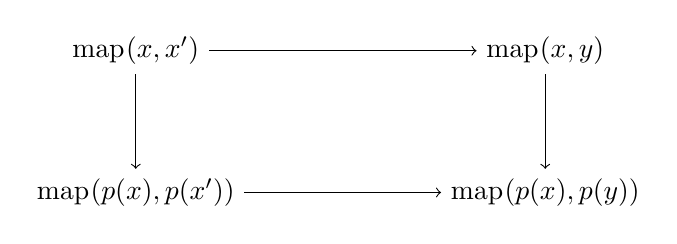
\begin{tikzpicture}
  \node (tl) at (0,0) {$\mathrm{map}_{\E}(x, x')$};
  \node (tr) at (5.2,0) {$\mathrm{map}_{\E}(x, y)$};
  \node (bl) at (0,-1.8) {$\mathrm{map}_{\C}(p(x), p(x'))$};
  \node (br) at (5.2,-1.8) {$\mathrm{map}_{\C}(p(x), p(y))$};
  \draw[->] (tl) -- (tr);
  \draw[->] (tl) -- (bl);
  \draw[->] (tr) -- (br);
  \draw[->] (bl) -- (br);
\end{tikzpicture}
\end{center}
从而诸竖直\trFibre{}间的诱导映射，是在对应于 $\mathrm{id}_{p(x)}$ 的那个点
$\Delta^0 \to \allowbreak \mathrm{map}_{\C}(p(x), p(x'))$ 之上的一个%
\trEquivalence{}。由
\cref{cor:mapping-homotopy-cartesian}，左边的竖直\trFibre{}由
$\mathrm{map}_{\E_{p(x)}}(x, x')$ 给出，断言即得。
\end{proof}

因此，拥有充足笛卡尔\trMorphism{}供给的\trInnerFibration{} $p\colon \E \to \C$
使得 $\E$ 中的诸\trMappingSpace{}由 $\C$ 的那些\trMappingSpace{}与所有%
\trFibre{}共同控制。

\begin{definition}\label{def:cartesian-cocartesian-fibration}
一个\trInnerFibration{} $p\colon X \to Y$ 称为一个%
\emph{\trCartesianFibration{}}（cartesian fibration），如果每个形如下述图表的%
\trLiftingProblem{}%
\begin{center}
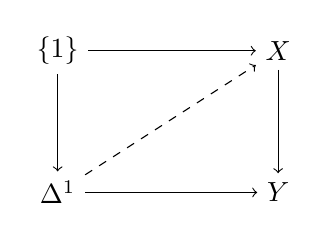
\begin{tikzpicture}
  \node (tl) at (0,0) {$\{1\}$};
  \node (tr) at (2.8,0) {$X$};
  \node (bl) at (0,-1.8) {$\Delta^1$};
  \node (br) at (2.8,-1.8) {$Y$};
  \draw[->] (tl) -- (tr);
  \draw[->] (tl) -- (bl);
  \draw[->] (tr) -- (br);
  \draw[->] (bl) -- (br);
  \draw[->, dashed] (bl) -- (tr);
\end{tikzpicture}
\end{center}
都容有一个解，且该解是 $X$ 中的一个 $p$-笛卡尔\trMorphism{}。对偶地，称 $p$
为一个 \emph{\trCocartesianFibration{}}（cocartesian fibration），如果每个形如
下述图表的\trLiftingProblem{}%
\begin{center}
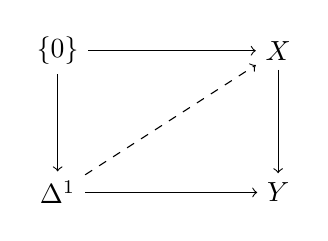
\begin{tikzpicture}
  \node (tl) at (0,0) {$\{0\}$};
  \node (tr) at (2.8,0) {$X$};
  \node (bl) at (0,-1.8) {$\Delta^1$};
  \node (br) at (2.8,-1.8) {$Y$};
  \draw[->] (tl) -- (tr);
  \draw[->] (tl) -- (bl);
  \draw[->] (tr) -- (br);
  \draw[->] (bl) -- (br);
  \draw[->, dashed] (bl) -- (tr);
\end{tikzpicture}
\end{center}
都容有一个解，且该解是 $X$ 中的一个 $p$-余笛卡尔\trMorphism{}。
\end{definition}

非正式地说，一个\trInnerFibration{}是一个（余）\trCartesianFibration{}，如果它
容有 $Y$ 中任何\trMorphism{}的一个 $p$-(余)笛卡尔提升（带有指定的源或目标）。%
\footnote{译注：原书此处印作「$\mathcal{C}$ 中的任何态射」（any morphism in
$\mathcal{C}$），但本定义中并未出现 $\mathcal{C}$——基是 $Y$；当系沿袭以
$\mathcal{C}$ 为基的记号之笔误，兹改为「$Y$ 中任何态射」。——译者注}

\begin{example*}
\trRightFibration{}是\trCartesianFibration{}，而\trLeftFibration{}是%
\trCocartesianFibration{}。
\end{example*}

\begin{lemma}\label{lem:cartesian-fibration-isofibration}
设 $p\colon \E \to \C$ 是∞-\trCategories{}之间的一个（余）\trCartesianFibration{}。
那么 $p$ 是一个\trIsofibration{}。
\end{lemma}

\begin{proof}
这由\cref{lem:equivalence-cartesian} 得出，后者断言：一个\trEquivalence{}的
$p$-笛卡尔提升是一个\trEquivalence{}。
\end{proof}

\begin{lemma}\label{lem:cartesian-fibration-right-fibration}
一个\trCartesianFibration{} $\E \to \C$ 是一个\trRightFibration{}，当且仅当
$\E$ 中每个\trMorphism{}都是 $p$-笛卡尔的。对偶地，一个\trCocartesianFibration{}%
是一个\trLeftFibration{}，当且仅当 $\E$ 中每个\trMorphism{}都是 $p$-余笛卡尔的。
\end{lemma}

\begin{proof}
按定义，在\trCartesianFibration{}中，人们可以提升右外 $1$-\trHorn{}。若进而
$\E$ 中每个\trMorphism{}都是 $p$-笛卡尔的，则这恰恰是说，人们还可以提升所有
维数大于等于 $2$ 的右外\trHorn{}。反之，一个\trRightFibration{}容有定义中的
图表的某个提升，而由\trRightFibration{}的定义，每个\trMorphism{}都是
$p$-笛卡尔的。余笛卡尔纤维化的论证类似。
\end{proof}

\begin{proposition}\label{prop:cartesian-fibration-fibres-groupoids}
设 $p\colon \E \to \C$ 是∞-\trCategories{}之间的一个\trCartesianFibration{}。
那么，$p$ 是一个\trRightFibration{}，当且仅当对 $\C$ 的所有\trObject{} $x$，
诸\trFibre{} $\E_x = \E \times_{\C} \{x\}$ 都是∞-\trGroupoid{}。
\end{proposition}

\begin{proof}
\trRightFibration{}恰是诸\trFibre{}为∞-\trGroupoid{}的\trCartesianFibration{}。
反之，设 $p\colon \E \to \C$ 是诸\trFibre{}皆为∞-\trGroupoid{}的一个%
\trCartesianFibration{}。我们将证明每个\trMorphism{}都是 $p$-笛卡尔的，然后
诉诸\cref{lem:cartesian-fibration-right-fibration}。为此，设 $f\colon \Delta^1 \to \E$
是一个从 $x$ 到 $y$ 的\trMorphism{}，并选取 $p(f)$ 的一个以 $y$ 为目标的
$p$-笛卡尔提升 $\varphi$。我们考虑图表
\begin{center}
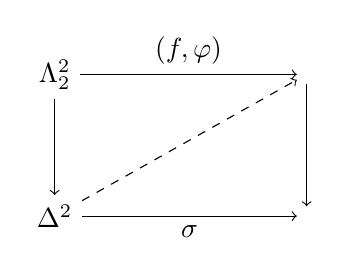
\begin{tikzpicture}
  \node (horn) at (0,0) {$\Lambda^2_2$};
  \node (e) at (3.2,0) {$\E$};
  \node (d2) at (0,-1.8) {$\Delta^2$};
  \node (c) at (3.2,-1.8) {$\C$};
  \draw[->] (horn) -- node[above] {$(f,\varphi)$} (e);
  \draw[->] (horn) -- (d2);
  \draw[->] (e) -- (c);
  \draw[->] (d2) -- node[below] {$\sigma$} (c);
  \draw[->, dashed] (d2) -- (e);
\end{tikzpicture}
\end{center}
其中映射 $\sigma$ 由图表
\begin{center}
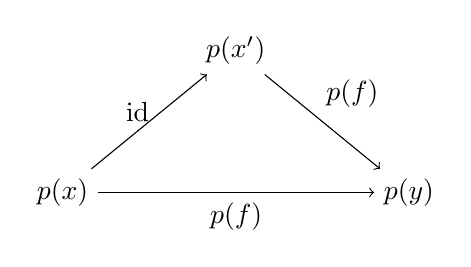
\begin{tikzpicture}
  \node (top) at (2.2,0) {$p(x')$};
  \node (bl) at (0,-1.8) {$p(x)$};
  \node (br) at (4.4,-1.8) {$p(y)$};
  \draw[->] (bl) -- node[above, pos=0.4] {$\mathrm{id}$} (top);
  \draw[->] (top) -- node[above right, pos=0.45] {$p(f)$} (br);
  \draw[->] (bl) -- node[below] {$p(f)$} (br);
\end{tikzpicture}
\end{center}
给出。由于 $\varphi$ 是 $p$-笛卡尔的，此图表中存在一条虚箭头。所得的
$2$-\trSimplex{} $\tau$ 由图表
\begin{center}
\begin{tikzpicture}
  \node (top) at (2.2,0) {$x'$};
  \node (bl) at (0,-1.8) {$x$};
  \node (br) at (4.4,-1.8) {$y$};
  \draw[->] (bl) -- node[above, pos=0.4] {$\psi$} (top);
  \draw[->] (top) -- node[above right, pos=0.45] {$\varphi$} (br);
  \draw[->] (bl) -- node[below] {$f$} (br);
\end{tikzpicture}
\end{center}
给出，其中 $\psi$ 是 $x$ 之上的\trFibre{} $\E_x$ 中的一个\trMorphism{}，从而由
诸\trFibre{}皆为∞-\trGroupoid{}的假设可知它是可逆的。于是，应用\cref{lem:cartesian-three-for-two}，我们发现 $f$ 是笛卡尔的，因为 $\varphi$
是。\footnote{译注：原书此二图中顶点 $1$ 分别印作 $p(y)$ 与 $y$——照录的话，
$\mathrm{id}$ 将成为 $p(x) \to p(y)$ 的边，而 $\varphi$ 与 $\psi$ 将成为 $y$
的自态射，两个图表都无法成立。按\trHorn{} $(f,\varphi)$ 的构成（边
$02 \mapsto f$、边 $12 \mapsto \varphi$）以及正文「$\psi$ 落在 $x$ 之上的%
\trFibre{} $\E_x$ 中」一语，顶点 $1$ 应为 $x'$（相应地 $p(x') = p(x)$），兹改之。
——译者注}
\end{proof}

\begin{remark}\label{rem:cartesian-fibration-fibres-groupoids-general}
\cref{prop:cartesian-fibration-fibres-groupoids} 的结论在 $\E$ 与 $\C$ 不被假设
为∞-\trCategories{}时也成立。事实上，人们可以由\cref{prop:cartesian-fibration-fibres-groupoids}
导出更一般的陈述，我们推荐把它当作一个练习来完成。
\end{remark}

\begin{corollary}\label{cor:cartesian-fibration-conservative}
一个\trCartesianFibration{}是\trConservative{}，当且仅当它是一个%
\trRightFibration{}。
\end{corollary}

\begin{proof}
由第 2 章中的\cref{prop:left-right-fibrations-conservative-isofibrations}，%
\trRightFibration{}是\trConservative{}。反之，给定一个\trConservative{}%
\trCartesianFibration{} $p\colon \E \to \C$，则 $\C$ 的每个\trObject{} $x$ 之上
的\trFibre{} $\E_x$ 是一个∞-\trGroupoid{}：\trFibre{}中的每个\trMorphism{}%
都被 $p$ 送到 $x$ 的恒等。于是我们可以应用\cref{prop:cartesian-fibration-fibres-groupoids}。
\end{proof}

\begin{definition}\label{def:morphism-of-fibrations}
设 $p\colon X \to Y$ 与 $p'\colon X' \to Y$ 是（余）\trCartesianFibration{}。我们称
一个映射 $f\colon X \to X'$ 为一个\emph{（余）\trCartesianFibration{}之间的%
\trMorphism{}}（morphism of (co)cartesian fibrations），如果 $p'f = p$，且 $f$
把 $p$-笛卡尔\trMorphism{}送到 $p'$-笛卡尔\trMorphism{}。
\end{definition}

\begin{example*}
设 $p\colon X \to Y$ 是一个\trCartesianFibration{}，而 $p'\colon X' \to Y$ 是一个%
\trRightFibration{}。那么任何满足 $p'f = p$ 的映射 $f\colon X \to X'$ 都是%
\trCartesianFibration{}之间的\trMorphism{}，因为 $X'$ 中的所有\trMorphism{}%
都是 $p'$-笛卡尔的。
\end{example*}

\begin{theorem}\label{thm:fibrewise-criterion}
设 $f\colon \E \to \E'$ 是（余）\trCartesianFibration{} $p\colon \E \to \C$ 与
$p'\colon \E' \to \C$ 之间的一个\trMorphism{}，其中诸\trCartesianFibration{}%
均介于∞-\trCategories{}之间。那么，$f$ 是一个\trJoyalEquivalence{}，当且仅当对
$\C$ 的所有\trObject{} $z$，诸\trFibre{}上的诱导映射 $\E_z \to \E'_z$ 是%
\trJoyalEquivalence{}。
\end{theorem}

\begin{proof}
「仅当」的方向对\trIsofibration{}之间的映射更一般地成立，见第 2 章中的%
\cref{lem:isofibration-fibrewise}。于是，让我们假设所有诱导映射
$\E_z \to \E'_z$ 都是\trJoyalEquivalence{}。我们希望证明 $f$ 是一个%
\trJoyalEquivalence{}。为此，我们将首先证明 $f$ 是\trFullyFaithful{}且%
\trEssentiallySurjective{}，然后由第 2 章中的\cref{thm:ffes-joyal-equivalence}
得出本定理。

为了看出 $f$ 是\trEssentiallySurjective{}，我们考虑 $\E'$ 的一个\trObject{}%
$y'$，并令 $x = p'(y')$。由于映射 $\E_x \to \E'_x$ 是一个\trJoyalEquivalence{}，
它特别地是\trEssentiallySurjective{}。于是，存在 $\E_x$ 中的一个\trObject{}%
$y$ 以及 $\E'_x$ 中 $f(y)$ 与 $y'$ 之间的一个\trEquivalence{}。由此可知 $f$
是\trEssentiallySurjective{}。

为了看出 $f$ 是\trFullyFaithful{}，我们考虑 $\E$ 中的两个\trObject{} $x$ 与
$y$，并需要证明映射
\[
\mathrm{map}_{\E}(x, y) \longrightarrow \mathrm{map}_{\E'}(f(x), f(y))
\]
是一个\trHomotopyEquivalence{}。

为此，取 $\alpha\colon x \to y$ 为 $\E$ 中的一个\trMorphism{}，并选取
$p(\alpha)$ 的一个 $p$-笛卡尔提升 $\hat{\alpha}\colon x' \to y$（这蕴含
$p(x') = p(x)$），同时注意，由假设 $f(\hat{\alpha})$ 是 $f(\alpha)$ 的一个
$p'$-笛卡尔提升。此外，由\cref{cor:cartesian-lift-mapping-fibre}，我们有%
\trHomotopy{}\trFibreSequence{}的图表
\begin{center}
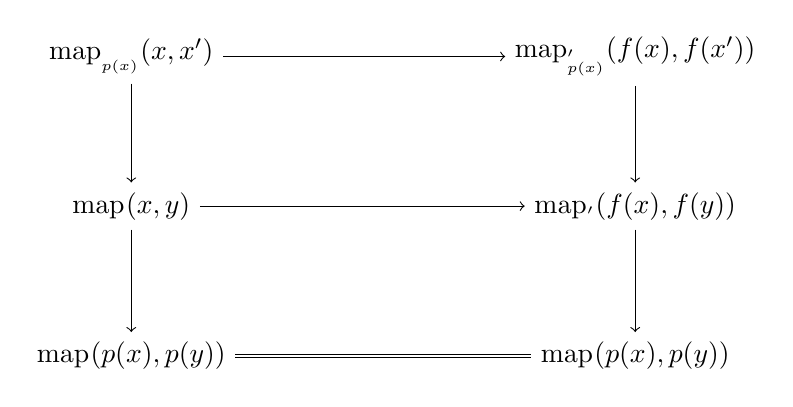
\begin{tikzpicture}
  \node (tl) at (0,0) {$\mathrm{map}_{\E_{p(x)}}(x, x')$};
  \node (tr) at (6.4,0) {$\mathrm{map}_{\E'_{p(x)}}(f(x), f(x'))$};
  \node (ml) at (0,-1.9) {$\mathrm{map}_{\E}(x, y)$};
  \node (mr) at (6.4,-1.9) {$\mathrm{map}_{\E'}(f(x), f(y))$};
  \node (bl) at (0,-3.8) {$\mathrm{map}_{\C}(p(x), p(y))$};
  \node (br) at (6.4,-3.8) {$\mathrm{map}_{\C}(p(x), p(y))$};
  \draw[->] (tl) -- (tr);
  \draw[->] (ml) -- (mr);
  \draw[double] (bl) -- (br);
  \draw[->] (tl) -- (ml);
  \draw[->] (tr) -- (mr);
  \draw[->] (ml) -- (bl);
  \draw[->] (mr) -- (br);
\end{tikzpicture}
\end{center}
其中基上的水平映射与\trFibre{}上的水平映射都是\trEquivalence{}，这由 $f$ 在诸%
\trFibre{}上的限制是\trFullyFaithful{}\trFunctor{}这一假设而知。于是，由第 2 章
中的\cref{lem:fibre-wise-homotopy-equivalence}，中间的水平映射也是%
\trEquivalence{}。\footnote{译注：原书未先行引入 $\alpha$，径谓「选取 $\alpha$
的一个 $p$-笛卡尔提升 $\hat{\alpha}$」——照录则 $\alpha$ 无定义（提升只能就基
中的边而言）；按上下文，$\alpha$ 应为 $\E$ 中任一边 $x \to y$，而 $\hat{\alpha}$
提升的是 $p(\alpha)$，兹补明。——译者注}
\end{proof}
